\documentclass[11pt]{article}
\usepackage{euscript}

\usepackage{amsmath}
\usepackage{amsthm}
\usepackage{amssymb}
\usepackage{epsfig}
\usepackage{xspace}
\usepackage{color}
\usepackage{url}
\usepackage[shortlabels]{enumitem}


%%%%%%%  For drawing trees  %%%%%%%%%
\usepackage{tikz}
\usetikzlibrary{calc, shapes, backgrounds}

%%%%%%%%%%%%%%%%%%%%%%%%%%%%%%%%%
\setlength{\textheight}{9in}
\setlength{\topmargin}{-0.600in}
\setlength{\headheight}{0.2in}
\setlength{\headsep}{0.250in}
\setlength{\footskip}{0.5in}
\flushbottom
\setlength{\textwidth}{6.5in}
\setlength{\oddsidemargin}{0in}
\setlength{\evensidemargin}{0in}
\setlength{\columnsep}{2pc}
\setlength{\parindent}{1em}
%%%%%%%%%%%%%%%%%%%%%%%%%%%%%%%%%


\newcommand{\eps}{\varepsilon}

\renewcommand{\c}[1]{\ensuremath{\EuScript{#1}}}
\renewcommand{\b}[1]{\ensuremath{\mathbb{#1}}}
\newcommand{\s}[1]{\textsf{#1}}

\newcommand{\E}{\textbf{\textsf{E}}}
\renewcommand{\Pr}{\textbf{\textsf{Pr}}}

\title{Homework 1 - Decision Trees
	\footnote{\s{CS 6350 Machine Learning; \;\; Spring 2024 \hfill
			Instructor: Vivek Kumar, University of Utah}
	}
}
\author{Cristian Tapiero}

\begin{document}
	\maketitle
	
	
	
	
	
	%%%%%%%%%%%%%%%%%%%%%%%%%%%%%%%%%%%%%%%%%%%%%%%%%%%%
	%%%%%%%%%%%%%%%%%%%%%%%%%%%%%%%%%%%%%%%%%%%%%%%%%%%%
	%%%%%%%%%%%%%%%%%%%%%%%%%%%%%%%%%%%%%%%%%%%%%%%%%%%%
	\section{Decision Trees}
	1.
	\begin{enumerate}[(a)] % (a), (b), (c), ...
		\item the total number of rows for the given attributes is $3\times3\times2\times2 = 36.$  
		So if we consider the values to be binary  there are $2^{36}$ possible functions.
		
		The number of functions that are consistent with the table given is $1.$
		
		\item Entropy is defined as $$H(S) =-p_+ log (p_+)-p_- log(p_-)$$
		
		Because $p_+ = p_- = 1/2$ Therefore, $H(S) = 1$
		
		\item Gain is defined as: $$\textit G(S,A) = Entropy(S) - \sum_{v\in Values(A)} \frac{|S_v|}{|S|} Entropy(S_v)$$ 
		
		As an example of the calculation, select A as the attribute Variety.
		$$\textit A = \{Alphonso,Keith,Haden\}$$
		
		First we calculate the Entropy for each of the subsets of the attribute Variety:
		
		$$\textit Entropy(Alphonso) = - \frac{1}{2}log(\frac{1}{2}) - \frac{1}{2}  log(\frac{1}{2}) = 1$$
		
		$$\textit Entropy(Keith) = -\frac{1}{3}log -\frac{2}{3} log(\frac{2}{3}) = 0.9118$$
		
		$$\textit Entropy(Haden) = -1log(1) - 0 log(0) = 0$$
		
		Then we compute the average part of the equation or the expected Entropy:
		$$\textit E(Entropy_{variety}) = 1 \times \frac{4}{8} + 0.918\times \frac{4}{8} + 0 \times \frac{1}{8} = 0.844$$
		
		Finally we calculate the Gain by subtracting the above value from the total entropy of the data set:
		$$\textit G(S,Variety) =  1 - 0.844 = 0.156 $$
		
		a similar procedure is applied to calculate the remaining gains for the other attributes given. The remaining results are presented in table 1.
		
		\begin{align}
			\begin{array}{cc}
				\hline \hline \text { Feature } & \text { Information Gain } \\
				\hline 
				Variety & 0.156  \\
				Color & 0.062  \\
				Smell & 0.189  \\
				Time & 0.049  \\
				\hline
			\end{array}
		\end{align}
		
		\begin{center} Table 1. Information Gain \end{center}
	
	\item I would use the Smell attribute to construct the root of the tree because is the highest value in table 1.
	\item The following tree represents the data given, choosing Smell as the root.
	\begin{center}
	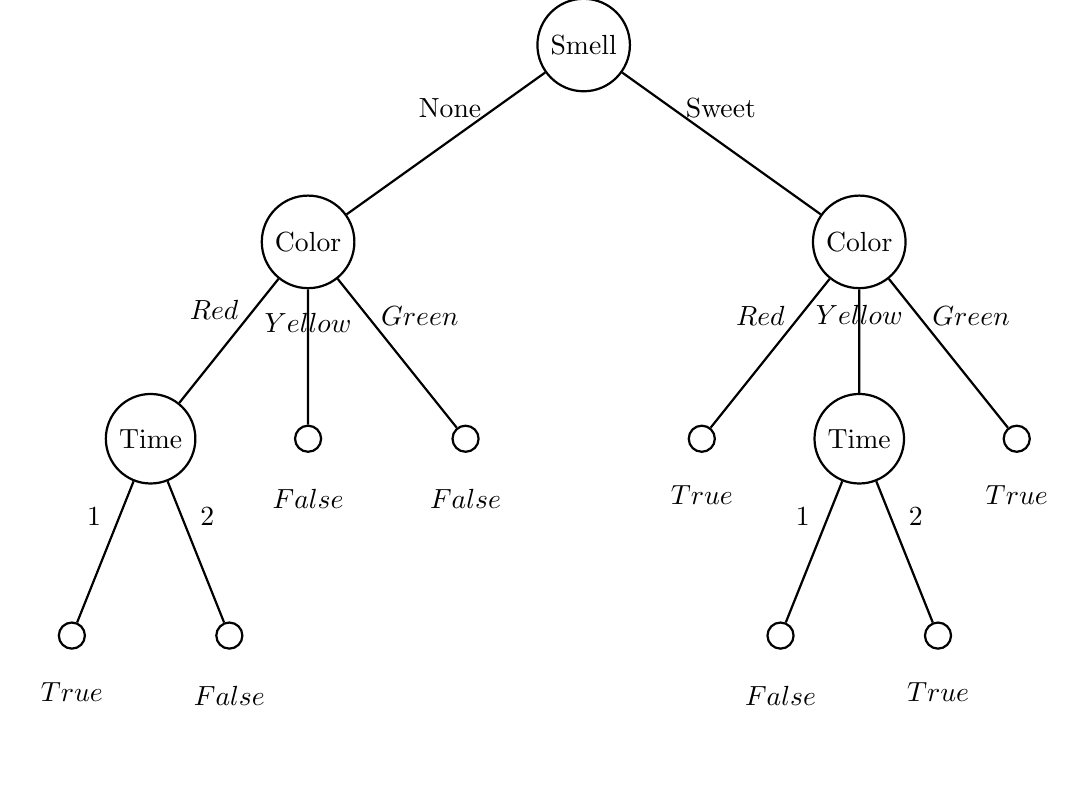
\begin{tikzpicture}[
		scale = 1, transform shape, thick,
		every node/.style = {draw, circle},
		grow = down,  % alignment of characters
		level 1/.style = {sibling distance=7cm},
		level 2/.style = {sibling distance=2cm}, 
		level distance = 2.5cm
		]
		\node (Start) { Smell} 
		child {   node (A) {Color}
			child { node (B) {Time} child{node (K) {}} child{node (J) {}}}
			child { node (C) {} }
			child { node (D) {}}
		}
		child {   node (E) {Color}
			child { node (F) {}}
			child { node (G) {Time} child{node (L) {}} child{node (M) {}}}
			child { node (H) {}}
		};
		
		
		% Put probability on edges
		\begin{scope}[nodes = {draw = none}]
			\path (Start) -- (A) node [near start, left]  {None};
			\path (A)     -- (B) node [near start, left]  {$Red$};
			\path (B)     -- (K) node [near start, left]  {$1$};
			\path (B)     -- (J) node [near start, right]  {$2$};
			\path (A)     -- (C) node [near start] {$Yellow$};
		    \path (A)     -- (D) node [near start,right] {$Green$};
			\path (Start) -- (E) node [near start, right] {Sweet};
			\path (E)     -- (F) node [near start, left]  {$Red$};
			\path (E)     -- (G) node [near start] {$Yellow$};
			\path (G)     -- (L) node [near start,left] {$1$};
			\path (G)     -- (M) node [near start,right] {$2$};
			\path (E)     -- (H) node [near start, right] {$Green$};
			\begin{scope}[nodes = {below = 4pt}]

				\node at (C) {$False$};
				\node at (D) {$False$};
				\node at (F) {$True$};
				\node at (H) {$True$};
				\node at (K) {$True$};
				\node at (J) {$False$};
				\node at (L) {$False$};
				\node at (M) {$True$};
			\end{scope}
		\end{scope}
	\end{tikzpicture}
	\end{center}
	
	\begin{center} Figure 1. Decision Tree \end{center}
	
	$\newline$
		\item using the decision tree on figure 1 we get the following predictions listed as a the last column in table 2
	
	\begin{align}
		\begin{array}{cccccc}
			\hline \hline \text { Variety } & \text { Color } & \text { Smell } & \text { Time } & \text { Ripe? } & \text { Predicted Label } \\
			\hline 
			Alphonso & Green & Sweet & Two & True & True \\
			Keitt & Red & Sweet & One & False  & True\\
			Haden & Yellow & None & Two & True &False\\
			\hline
		\end{array}
	\end{align}
	
	\begin{center} Table 2. Predicted Values \end{center}
	
	We can calculate the Accuracy of the classifier as follows:
	
	$$Accuracy =( 
	\displaystyle\frac{\text{ Number of Correct Predictions}}{\text
		{Number of Predictions}}) \times 100$$
	
	Therefore, only having 1 correct prediction give an accuracy of about 33.33\%
	
	

	\end{enumerate}
2.
	\begin{enumerate}[(a)]
		\item  the New Information Gain is defined as: $$\textit G(S,A) = MajorityError(S) - \sum_{v\in Values(A)} \frac{|S_v|}{|S|} MajorityError(S_v)$$ 
		where MajorityError is defined as:
		$$\textit MajorityError(S) = 1 - max_ip_i$$ 
		$$\textit MajorityError(S_v) = 1 - max_ip_{i,v}$$ 
		
		\item As an example of the calculation, select A as the attribute Color.
		$$\textit A = \{Alphonso,Keith,Haden\}$$
		
		First we calculate the the Majority error for each of the subsets of the attribute Color:
		
		$$\textit MajorityError(Red) = 1 - \frac{2}{3} = \frac{1}{3}$$ 
		where  $\frac{2}{3}$ is $max_ip_{i,v}$
		
		$$\textit MajorityError(Yellow) = 1 - \frac{2}{3} = \frac{1}{3}$$ 
		where  $\frac{2}{3}$ is $max_ip_{i,v}$
		
		$$\textit MajorityError(Green) = 1 - \frac{1}{2} = \frac{1}{2}$$ 
		where  $\frac{1}{2}$ is $max_ip_{i,v}$
		
		Then we compute the average part of the equation or the expected Majority Error:
		$$\textit E(MajorityError_{variety}) = \frac{3}{8} \times \frac{1}{3} + \frac{3}{8} \times \frac{1}{3} + \frac{2}{8} \times \frac{1}{2} = \frac{3}{8}$$
		
		Finally we calculate the Gain by subtracting the above value from the MajorityError of the entire set:
		$$\textit G(S,Variety) =  \frac{1}{2} - \frac{3}{8} = \frac{1}{8}  \approx 0.125
		 $$
		
		a similar procedure is applied to calculate the remaining gains for the other attributes given. The remaining results are presented in table 3.
		
		\begin{align}
			\begin{array}{cc}
				\hline \hline \text { Feature } & \text { Information Gain } \\
				\hline 
				Variety & 0.125  \\
				Color & 0.125  \\
				Smell & 0.250  \\
				Time & 0.125  \\
				\hline
			\end{array}
		\end{align}
		
		\begin{center} Table 3. Information Gain using Majority Error Function \end{center}
		\item According to my results the attribute that will become the root node of the decision tree will be Smell. So both measurements  (Entropy and majority error) lead to the same root but not necessarily the same tree.
		\end{enumerate}
\section{Experiments}

\subsection*{1. baseline}
	\begin{enumerate}
		\item The most common label in the training set is "e" or edible.The accuracy of a classifier that uses only that label to predict the outcome on the training and test data is given by the equation:
		$$ accuracy = \frac{\# \text{ of correct predictions }}{\# \text{ total predictions}}  \times 100$$
		
		For the Training data the number of "e" labels  is 3392 and the total number of predictions is 6530 giving an Accuracy of 0.517 or $\approx 52\%$
		
		Similarly the Test data has 3382 "e" labels and the total of predictions is 6530 giving a similar accuracy of 0.517 or $\approx 52\%$
	\end{enumerate}
\subsection*{2. Implementation: Full Tree}
	In the implementation of the ID3 algorithm I created a class called desicionTree which represents a node in the tree. Each node in the tree contains information such as its name, label (if it's a leaf node), information gain, branches (child nodes), and the feature it's split on. For the branches I decided to use a dictionary which key represents the attribute the algorithm splits and the values of the key as the possible values this attribute can take.
	My code is structured in a way that combines functions and classes to promote code reuse and modularity. The  main function or the entry point of the program (located at the bottom of the file) calls the ID3 function which returns a tree object. Using the function validate I calculate the accuracy of the predictions.
	ID3 and validate also call other helper functions that provide calculations needed on their function bodies respectively.
	(As a clarification the ? values in the data were replaced with the most common label in that column)
	\begin{enumerate}[(a)]
		
		\item The root feature selected by my ID3 algorithm was \textbf{spore-print-color}
		\item The Information gain of the root node is \textbf{0.845} 
		\item  The Maximum Depth of the Tree is \textbf{7}
		\item The accuracy of the Training set is \textbf{100\%}
		\item The accuracy of the Test set is \textbf{100\%}
	\end{enumerate}

\subsection*{3. Limiting Depth}

	For this implementation I implemented a function called k-foldvalidation which takes as inputs an Array and the depth.The array is later iterated over to get the different possible combinations of training and validation sets. (As a clarification the ? values in the data were replaced with the most common label in that column)   
	\begin{enumerate}[(a)]
		
		\item \begin{align}
			\begin{array}{ccc}
				\hline \hline \text { Depth } & \text { Average Cross Validation } & {Standard Deviation} \\
				\hline 
				1 & 0.518 & 0.306\\
				2 & 0.523 & 0.300\\
				3 & 0.810 & 0.147\\
				4 & 0.943 & 0.043\\
				5 & 0.954 & 0.033\\
				10 & 0.964 & 0.033 \\
				15 & 0.964 & 0.033  \\
				\hline
			\end{array}
		\end{align}
		\begin{center} Table 4. Average cross validation and standard deviation of k-fold cross-validation  \end{center}
		The depth that is best from the set is 5 because is closer to a probability of 1. That being said the full tree already reaches 100\% accuracy so it will be a second best. Depths 10 and 11 are not attainable because the max depth of the full tree is 7.
		 
		\item  I implemented the depth limit functionality as a parameter to the function ID3 in which  two parameters are incorporated directly into the function logic. The depth of each node is incremented during each recursive call. When the depth reaches the specified limit (max depth), the recursion stops, limiting the depth of the decision tree.
		
		\item  The Accuracy for depth 5 on the test data is 0.981
		
		\item The performances of the depth limited tree and the full decision tree are similar. This is because as mentioned before the full tree gives already 100\% accuracy. That being said if we can achieve pretty good accuracy with a shorter tree it is better to use it because with a full tree we run the risk of overfitting our data. By limiting the depth, the tree is less likely to capture noise or outliers in the data, resulting in improved generalization performance. Additionally a smaller tree requires less computation power than its counter part if we were to build our model on big data.
		
		
		
	\end{enumerate}
\section{Decision Trees with Attribute Costs}
	\begin{enumerate}
		
		\item Information Gain is defined as: $$\textit G(S,A) = Entropy(S) - \sum_{v\in Values(A)} \frac{|S_v|}{|S|} Entropy(S_v)$$ 
		
		First we calculate the Entropy of the entire set $H(S)$:
		
		$$\textit Entropy(S) = - \frac{7}{12}log(\frac{7}{12}) - \frac{5}{12}  log(\frac{5}{12}) = 0.98$$
		
		As an example of the calculation, select A as the attribute Color.
		$$\textit A = \{Red,Blue,Yellow,Pink\}$$
		
		Then we calculate the Entropy for each of the subsets of the attribute Variety:
		
		$$\textit Entropy(Red) = - \frac{1}{2}log(\frac{1}{2}) - \frac{1}{2}  log(\frac{1}{2}) = 1$$
		
		$$\textit Entropy(Blue) = -\frac{4}{5}log(\frac{4}{5}) -\frac{1}{5} log(\frac{1}{5}) = 0.722$$
		
		$$\textit Entropy(Yellow) = - \frac{1}{3}log(\frac{1}{3}) - \frac{2}{3}  log(\frac{2}{3}) = 1$$
		
		$$\textit Entropy(pink) = -1log(1) - 0 log(0) = 0.918 $$
		
		Then we compute the average part of the equation or the expected Entropy:
		$$\textit E(Entropy_{variety}) = 1 \times \frac{2}{12} + 0.722\times \frac{5}{12} + 1 \times \frac{2}{12} + 0.918\times \frac{3}{12} = 0.864$$
		
		Then we calculate the Gain by subtracting the above value from the total entropy of the data set:
		$$\textit G(S,Variety) =  0.98 - 0.864 = 0.116 $$
		
		Finally, we have the definition of $Gain_T$ and $Gain_N$
				$$Gain_T(S,A) = \frac{Gain(S,A)^2}{Cost(A)} $$
		and

		\[Gain_N(S,A) = \frac{2^{Gain(S,A)} - 1}{Cost(A) + 1}\] 
		
		and calculate them respectively:
		$$Gain_T(S,A) = \frac{0.116)^2}{30)} = 0.000449 $$
		\[Gain_N(S,A) = \frac{2^{0.116} - 1}{30) + 1} = 0.015\]
			
		a similar procedure is applied to calculate the remaining gains for the other attributes given. The remaining results are presented in table 5.
		
		
		
		\begin{align}
			\begin{array}{ccc}
				\hline \hline \text { Attribute } & \mathnormal{Gain_t}& \mathnormal{Gain_n} \\
				\hline 
				Shape & 0.000384 & 0.013\\
				Color & 0.000449 & 0.015\\
				Size & 0.000571 & 0.017\\
				Material & 0.000353 & 0.014\\
				\hline
			\end{array}
		\end{align}
		\begin{center} Table 5. Information Gain with costs  \end{center}
		\item For $Gain_T$ I would choose the Attribute size  and for $Gain_N$ I would choose Size aswell.
	\end{enumerate}
	
\end{document}
